%%%%%%%%%%%%%%%%%%%%%%%%%%%%%%%%%%%%%%%%%
% University Assignment Title Page 
% LaTeX Template
% Version 1.0 (27/12/12)
%
% This template has been downloaded from:
% http://www.LaTeXTemplates.com
%
% Original author:
% WikiBooks (http://en.wikibooks.org/wiki/LaTeX/Title_Creation)
%
% License:
% CC BY-NC-SA 3.0 (http://creativecommons.org/licenses/by-nc-sa/3.0/)
% 
% Instructions for using this template:
% This title page is capable of being compiled as is. This is not useful for 
% including it in another document. To do this, you have two options: 
%
% 1) Copy/paste everything between \begin{document} and \end{document} 
% starting at \begin{titlepage} and paste this into another LaTeX file where you 
% want your title page.
% OR
% 2) Remove everything outside the \begin{titlepage} and \end{titlepage} and 
% move this file to the same directory as the LaTeX file you wish to add it to. 
% Then add \input{./title_page_1.tex} to your LaTeX file where you want your
% title page.
%
%%%%%%%%%%%%%%%%%%%%%%%%%%%%%%%%%%%%%%%%%
%\title{Title page with logo}
%----------------------------------------------------------------------------------------
%	PACKAGES AND OTHER DOCUMENT CONFIGURATIONS
%----------------------------------------------------------------------------------------

\documentclass[10pt]{article}
\usepackage[english]{babel}
\usepackage[utf8x]{inputenc}
\usepackage[table]{xcolor}
\usepackage{amsmath}
\usepackage{graphicx}
\usepackage{amssymb}
% \usepackage[shortlabels]{enumitem}
\usepackage{enumitem}
\usepackage[colorinlistoftodos]{todonotes}
\usepackage{ntheorem}
\usepackage[toc,page]{appendix}
\usepackage{geometry}
\usepackage{algpseudocode}
\usepackage{algorithm}
\usepackage{wrapfig}
\usepackage{color, colortbl}
\definecolor{Gray}{gray}{0.9}
\definecolor{DarkGray}{rgb}{0.75,0.75,0.75}
\newcolumntype{g}{>{\columncolor{Gray}}c}
\usepackage{multirow}
\usepackage{sidecap}
\usepackage{wrapfig}
\geometry{a4paper, left=20mm, top=20mm, right = 20mm}

\usepackage{listings}
\usepackage{color}
\usepackage{mathtools}
\DeclarePairedDelimiter\ceil{\lceil}{\rceil}
\DeclarePairedDelimiter\floor{\lfloor}{\rfloor}
\usepackage[font={small}]{caption}
\usepackage{subcaption}
\setlength{\abovedisplayskip}{4pt}
\setlength{\belowdisplayskip}{4pt}
%\usepackage{minted}
\usepackage{url}
\setlength{\parindent}{1em}
\setlength{\parskip}{0.5em}
\usepackage{multicol}

\begin{document}

\noindent
\textbf{Franziska Riegger} \hfill \textbf{August 14, 2020}\\[0.1cm]
% \normalsize ETHZ 19-904-580 \hfill Final Assignment\\
\newcommand{\HRule}{\rule{\linewidth}{0.5mm}} % Defines a new command for the horizontal lines, change thickness here

% \center % Center everything on the page
 \begin{center}
%----------------------------------------------------------------------------------------
%	HEADING SECTIONS
%----------------------------------------------------------------------------------------

% \textsc{\LARGE University of Utrecht}\\[1.5cm] % Name of your university/college
% \textsc{\Large Parallel Algorithms - Assignment 1}\\[0.5cm] % Major heading such as course name
% \textsc{\large Assignment 1}\\[0.5cm] % Minor heading such as course title

%----------------------------------------------------------------------------------------
%	TITLE SECTION
%----------------------------------------------------------------------------------------

\HRule \\[0.4cm]
\textsc{\Huge Inverse Theory}\\[0.25cm]
\textsc{\Large Optimized HIV drug treatment using probabilistic inversion}
\\[0.2cm] % Title of your document
\HRule \\[1.0cm]
 
%----------------------------------------------------------------------------------------
%	AUTHOR SECTION
%----------------------------------------------------------------------------------------

% \Large \emph{Author:}\\
% Franziska \textsc{Riegger} (TU Delft - 4958950)\\[1.0cm] % Your name

%----------------------------------------------------------------------------------------
%	DATE SECTION
%----------------------------------------------------------------------------------------

% {\large October 17, 2018}\\[1.0cm] % Date, change the \today to a set date if you want to be precise

%----------------------------------------------------------------------------------------
%	LOGO SECTION
%----------------------------------------------------------------------------------------

% \includegraphics[width=0.2\textwidth]{images/logo-mastermath.jpeg}\\[1cm] % Include a department/university logo - this will require the graphicx package
 
%----------------------------------------------------------------------------------------
% \begin{abstract}

During the last 40 years, \textit{Human Immunodeficiency Viruses}, short HIV, has been a permanent companion of human mankind.
In the recent past, mortality rate could be decreased thanks to highly developed drugs.
However, still patients might suffer from strong side effects which again lower their life quality.
This report aims on developing a methodology to individually tailor kind and dose of antiretroviral treatment to each patient.
In a first step, an approach how to quantify the efficiency of a drug is introduced.
By defining a set of ODEs this metric can be indirectly correlated to observable viral load within the blood plasma of the patient.
In order to infer statements about the drug's efficiency based on observations, the problem is formulated as a Bayes inversion problem.
Prior knowledge about the model and observations is represented by probability distributions which can be used to find a non-explicit definition of the posterior probability distribution of the model.
Using a Simulated Annealing algorithm allows to sample from this posterior distribution in order to find the model with maximal posterior likelihood.
Based on this, the efficiency of the drug is computed and the therapy either accepted or rejected and a new medication tried.

\end{abstract}
% \vfill % Fill the rest of the page with whitespace
% \end{titlepage}

\end{center}

% \section*{Table of Content}
\subsection*{Proposal 1}

\begin{enumerate}[font=\bfseries]
    \item \textbf{Introduction}
    \item \textbf{The Dynamic HIV Model}
    \begin{itemize}[font=\small]
        \item \textit{(short) Model review}: Linear/nonlinear; Different models simulate different interactions, 
        cell popultaions, virus developments (e. g. resistance) etc.
        \item \textit{Model requirements}: What should our model be capable of simulating?
        \item \textit{Model definition/selection}: Introduce a modified version of the model in \cite{wu2010game}; 
        Which modifications and why?; Introduce all parameters (biological meaning + reference values \cite{adams2005hiv} + units) and state 
        which have to be estimated from patient's data \cite{callaway2002hiv}
    \end{itemize}
    \item \textbf{The Clinical Data}
    \begin{itemize}[font=\small]
        \item \textit{Numerical simulation}: Predefine a set of true parameters, including initial drug dosages; Interprete a set of numerical results as a sequence of blood 
        tests (e.g. every other day within the first 8 weeks)
    \end{itemize}
    \item \textbf{The Methods to Personalize the Model}
    \begin{enumerate}[font=\bfseries]
        \item \textbf{Probabilistic Formulation of Prior Knowledge and Bayes' Theorem}
        \begin{itemize}[font=\small]
            \item \textit{Prior Knowledge in Data Space}: clinical data suffers from measurement errors (e.g. environment of blood tests can 
            not accurately be reconstructed, different time intervals elapsed between blood test and evaluation, uncertainties in instruments 
            used to evaluate viral load etc.); blood tests are independent samples; cells counts can only be positive and change fast in the 
            first weeks of the treatment
            \item \textit{Prior Knowledge in Data Space}: Any biological contraints on parameters? Is there a reference value and how strong
            are the expected deviations from it?
            \item \textit{Bayes' Theorem}
        \end{itemize}
        \item \textbf{Sampling with Markov Chain Monte Carlo Method}
        \begin{itemize}[font=\small]
            \item \textit{Implementation Details}
        \end{itemize}
    \end{enumerate}
    \item \textbf{Results and Discussion}
    \item \textbf{Summary and Outlook}
    \begin{itemize}[font=\small]
        \item \textit{Outlook}: this personalized dynamic model can be used to solve an optimal control problem to find ideal drug dosages
    \end{itemize}
\end{enumerate}

\subsection*{Proposal 2}
More comprehensive alternative: the focus might not only be on the inversion but the additional sections for Optimal Control won't 
go into detail and only introduce the broad idea


\begin{enumerate}[font=\bfseries]
    \item \textbf{Introduction}
    \item \textbf{The Model for a Personalized HIV Treatment}
    \begin{enumerate}[font=\bfseries]
        \item \textbf{The Dynamic Model}
        \begin{itemize}[font=\small]
            \item \textit{see Proposal 1}
        \end{itemize}
        \item \textbf{The Optimal Control Problem}
        \begin{itemize}[font=\small]
            \item \textit{Control Parameter}: drug dosages
            \item \textit{Cost function}: define the cost function which has to be maximized in order to minimize the side effects
        \end{itemize}
    \end{enumerate}
    \item \textbf{The Clinical Data}
    \begin{itemize}[font=\small]
        \item \textit{see Proposal 1}
    \end{itemize}
    \item \textbf{The Methods}
    \begin{enumerate}[font=\bfseries]
        \item \textbf{Personalized Model - Bayesian Approach for Parameter Estimation}
        \begin{itemize}[font=\small]
            \item \textit{see Methods section of Proposal 1}
        \end{itemize}
        \begin{enumerate}[font=\bfseries]
            \item \textbf{Probabilistic Formulation of Prior Knowledge and Bayes' Theorem}
            \item \textbf{Sampling with Markov Chain Monte Carlo Methods}
        \end{enumerate}
        \item \textbf{Adjusted drug dose - Optimal control}
        \begin{itemize}[font=\small]
            \item \textit{Computing optimal controls}: state idea of Pontryagin's Maximum Principle
        \end{itemize}
    \end{enumerate}
    \item \textbf{Results and Discussion}
    \begin{itemize}[font=\small]
        \item focus on parameter estimation
    \end{itemize}
    \item \textbf{Summary and Outlook}
\end{enumerate}
% \begin{abstract}

During the last 40 years, \textit{Human Immunodeficiency Viruses}, short HIV, has been a permanent companion of human mankind.
In the recent past, mortality rate could be decreased thanks to highly developed drugs.
However, still patients might suffer from strong side effects which again lower their life quality.
This report aims on developing a methodology to individually tailor kind and dose of antiretroviral treatment to each patient.
In a first step, an approach how to quantify the efficiency of a drug is introduced.
By defining a set of ODEs this metric can be indirectly correlated to observable viral load within the blood plasma of the patient.
In order to infer statements about the drug's efficiency based on observations, the problem is formulated as a Bayes inversion problem.
Prior knowledge about the model and observations is represented by probability distributions which can be used to find a non-explicit definition of the posterior probability distribution of the model.
Using a Simulated Annealing algorithm allows to sample from this posterior distribution in order to find the model with maximal posterior likelihood.
Based on this, the efficiency of the drug is computed and the therapy either accepted or rejected and a new medication tried.

\end{abstract}
\section{Introduction}
\label{sec:Introduction}

From its first occurrence in the early beginning of the 1980s until this very day, \textit{Human Immunodeficiency Viruses}, widely known as HIV, has taken 39 million lives.
Thanks to enhanced prevention and highly sophisticated medication, the brutality of the pandemic has been remarkably reduced since its peak in 2004.
Although, nowadays numerous antiretroviral treatment exist, aiming on inhibiting the viruses, patients suffers from strong side effects.
Optimally, the choice of kind and dose of drug has to be made individually for each patient.
However, finding the perfect medication by trial and error is cumbersome and painful.\\
This scientific report is not only concerned with finding a metric to quantify the efficiency of HIV treatments but also develops a systematic approach how to derive this efficiency measure individually for each patient.\\ \\
% Nevertheless, for a profound understanding of the HIV infection and its antiviral treatment on a long-term scale, further HIV studies are necessary.
For this, Adames et. al \cite{ADAMS200510} suggest to model the dynamics of the viruses under the effect of an antiretroviral treatment by the following set of non-linear ODEs (\textit{Ordinary Differential Equations}): 

\begin{align}
    \begin{split}
        \dot{T} &= \lambda - \rho T - (1 - \gamma(t))kTV\\
        \dot{T}^{*} &= (1-\gamma(t))kTV-\delta T^{*}\\
        \dot{V} &= N\delta T^{*}-cV \quad \text{.}
    \end{split}
    \label{equ:ODEs}
\end{align}

Although, HIV has more than one potential target cell\footnote{Target cells are cells that are infected by HIV, mainly the helper T cells such as CD4+ T cells or macrophages.} the above model considers only the population of one, denoted by $T$.
$T^*$ describe the infected target cells which actively produces free viruses $V$. 
Further $\lambda$ in $\frac{cells}{day\cdot ml}$ represents the rate at which new $T$ cells are created from sources within the body, $\rho$ in $\frac{1}{day}$ is the death rate of $T$ cells, $k$ in $\frac{ml}{virions\cdot day}$ the rate by which $T$ cells are infected by virus, $\delta$ in $\frac{1}{day}$ is the death rate for infected cells , $N$ the number of new virions produced from each of the infected cells during their lifetime, and finally $c$ in $\frac{1}{day}$ is the clearance rate of free virions. 
The time-varying parameter $\gamma(t) \in [0,1]$ quantifies the antiviral drug efficacy whose formal definition will not be given here.
A drug is said to be efficient if all viruses are inhibited, i.e. $\gamma(t) = 1$.
Only if this is the case, the ODEs \ref{equ:ODEs} can be solved analytically, otherwise numerically.
In the following, we will assume an imperfect inhibition and denote the numerical solution of the viral load by $\tilde{V}_j \approx V(t_j)$ at time $t_j$ (the considered time period is discretized in $N_t$ time steps).
Further, Huang et. al claim that if $\gamma(t) > e_c$ for all $t$ the virus will be eventually eradicated.
Thus, the so-called \textit{efficacy threshold} $e_c$, defined as

\begin{align}
 e_c = 1-\frac{c\rho}{kN}\lambda
 \label{equ:e_c}
\end{align}

can be interpreted as the ability of a patient’s immune system to control viral replication.
For an optimized drug treatment it is important to know $e_c$ for each patient.
At the same time, only the viral load $V(t)$ can directly be measured in the blood plasma.
Hence, $e_c$ can only be retrieved by estimating the model parameters $\mathbf{m} = (c, \rho, k, N, \lambda)$ from the patient's clinical data  \cite{huang2003modeling}.\\
All in all, estimating the patient specific, discrete model parameter $\mathbf{m}$ is an inverse problem.
The associated forward problem is given by the set of equations \ref{equ:ODEs} which non-linearly relates the model parameter $\mathbf{m}$ to the observations $V_{obs}$.
\section{The Model for a Personalized HIV Treatment}
\label{sec:model}

In this section, we introduce a mathematical model that allows us to simulate the evolution of an HIV infection.
After further investigating this model and discussing the impact of antiretroviral drugs, the optimal control problem is formulated.

\subsection{The Dynamic Model}
\label{subsec:Model_DynModel}

Since HIV has first been simulated in the mid-90s, a wide variety of different models arose.
Initially, the latter attempted to investigate the HIV evolution by a set of linear \textit{ordinary differential 
equations} (ODEs). These however, are mere approximations of the realistic dynamics of viral pathogenesis and, hence only 
applicable for a short period of time, ranging in the orders of days.
HIV, treated or untreated, is a disease that extents over years and accurate and reliable long-term investigations 
require non-linear models \cite{adams2005hiv}.\newline
In addition hereto, the final model definition is determined by the choice of biological compartments and interactions 
that one wants to simulate.
Some models, for instance, differentiate between potential traget cells, usually including CD4+ T cells and macrophages \cite{perelson1993dynamics}.
Once a cell is infected, it can either remain in a latent state or actively reproduce new viral cells, causing different reaction of 
the patient’s immune system \cite{anderson1998complex}.\par

To optimize HAARTs, we require a model that does not only simulate the interaction between viral and immune cells but 
one that also considered the effect of the taken drugs.\newline
For this, we first have to review the working principle and impact of HAART.
% Finding such a model, demands for reviewing the working priciples of HAART.
Generally, this therapy is a combination of multiple classes of antiretroviral drugs, each fighting the virus in different ways.
Two of these are the so-called \textit{reverse transcriptase inhibitors} (RTIs) and the \textit{protease inhibitors} (PIs).
While the first aims at blocking the initial infection of target cells, the latter causes already infected cells to only produce 
immature virus.
Both these drugs, are solely designed for virus cells with a specific genome.
HIV, however, replicate in untreated persons at an exponentionally high rate, generating up to $10^{10}$ new free virus 
cells per day. Essential steps in this duplication are error-prone and hence, the probability of mutations is high.
The emerging cells have modified genomes, and the deployed drugs inhibt them less efficiently.
Thus, an appropriate model has to distiguish between drug-sensitive and resistant viruses \cite{rong2007emergence}.\par
According Rong et al. \cite{rong2007emergence}, a model that meets all our requirements, can be described by the following set 
of differential equations:

\begin{align}
    \begin{split}
        \dot{T}(t) &= \lambda - dT(t) - k_s (1 - \varepsilon_{RT}^s) V_s(t) T(t) - k_r (1 - \varepsilon_{RT}^r) V_r(t) T(t),\\
        \dot{T_s}(t) &= (1-u)k_s(1 - \varepsilon_{RT}^s)V_s(t)T(t) - \delta T_s(t),\\
        \dot{V_s}(t) &= N_s \delta (1 - \varepsilon_{PI}^s) T_s(t) - c V_s(t),\\
        \dot{T_r}(t) &= u k_s (1 - \varepsilon_{RT}^s) V_s(t) T(t) + k_r (1 - \varepsilon_{RT}^r) V_r(t) T(t) - \delta T_r(t),\\
        \dot{V_r}(t) &= N_r (1 - \varepsilon_{PI}^r) \delta T_r(t) - c V_r(t).
    \end{split}
    \label{equ:HIVmodel}
\end{align}

Here, $T(t)$ denotes the concentration of uninfected target T cells.
Generally, by index $s$ we denote the drug-sensitive strain whereas index $r$ marks the drug-resistant one.
% As discussed above, we are distiguishing between drug sensitive and resistant strains.
Thus, $T_s(t)$ is the concentration of cells that are infected by drug-sensitive viral cells $V_s(t)$.
$T_r(t)$ is the concentration of cells that are infected by drug-resistant viral cells $V_r(t)$.
Note, that all concentrations are given in $1/ml$.
The rate at which $T_s(t)$ cells become drug-resistant during the process of replication is given by the parameter $u$ ($0 \leq u < 1$).\newline
Further, $\lambda$ represents the birth rate of uninfected T cells per day, $d$ is their per capita daily death rate.
Apart from natural death, the T cell population is reduced by infection. $k_s$ and $k_r$ represent the constant rates at which 
uninfected cells are infected by drug sensitive and resistant virus, respectively.
At the same time, these rates are reduced by the use of RITs. The efficacy of the drug is given by the dimensionless 
parameters $\varepsilon_{RT}^{s}$ and $\varepsilon_{RT}^{r}$, both ranging between 0 and 1.
Since sensitive viruses are more susceptible to drugs, it is $\varepsilon_{RT}^{s} > \varepsilon_{RT}^{r}$.\newline
We assume that both kinds of infected cells, $T_s(t)$ and $T_r(t)$, burst and consequently die at the same daily rate $\delta$.
During bursting, a certain number of free virus cells are released. For sensitive virus cells, the number is denoted by $N_s$ 
while $N_r$ describes the same quantitiy in the drug-resistant case.
However, under the deployment of PIs, not all of the newly generated free virus cells are themselves capable of infecting healthy immune 
cells. This is encoded in the efficacy parameters $\varepsilon_{PI}^s$ and $\varepsilon_{PI}^r$. Again, it is $0 \leq \varepsilon_{PI}^s \leq 1$, 
$0 \leq \varepsilon_{PI}^r \leq 1$ and $\varepsilon_{PI}^s > \varepsilon_{PI}^r$.
Virus cell populations are only reduced by their daily clearance rate $c$.\newline
With the parameters $\varepsilon_{RT}$ and $\varepsilon_{PI}$, we describe the efficacy of the single antiretroviral drugs.
Summarizing these to the overall drug efficacy $\varepsilon = 1 - (1-\varepsilon_{RT})(1-\varepsilon_{PI})$ allows us to assess the efficacy of 
the combination therapy.
Hence, it is

\begin{align}
    \begin{split}
        \varepsilon_s &= 1 - (1-\varepsilon_{RT}^s)(1-\varepsilon_{PI}^s)\, ,\\
        \varepsilon_r &= 1 - (1-\varepsilon_{RT}^r)(1-\varepsilon_{PI}^r) \,\text{.}
    \end{split}
    \label{ref:epsilon_HAART}
\end{align}

In the following, we assume that the resistance level of the HIV mutants can be quantified by the parameter $\alpha\; (0 < \alpha < 1)$, 
which represents the reduction in drug efficacy by $\varepsilon_{s} = \alpha \varepsilon_{r}$.\newline
Descriptions and units of all parameters are summarized in table \ref{tab:init_parameters}.\par

\renewcommand{\arraystretch}{1.25}
\begin{table}
    \centering
    % \begin{tabular}{m{5em} m{10em} m{20em}}
        \begin{tabular}{ ccc }
        \hline
        \hline
        \multicolumn{3}{c}{\textit{Parameter definitions and values used in numerical simulation}} \\
        \hline
        % \rule{0pt}{10pt}
        Parameter & Value & Description\\[0.5ex]
        \hline
        $\lambda$   & $10^4\,\text{ml}^{-1}\text{day}^{-1}$ & Birth rate of uninfected cells\\
        $d$   & $0.01\,\text{day}^{-1}$  & Natural death rate of uninfected cells\\
        $k_s$   & $2.4 \times 10^{-8}\,\text{ml}\,\text{day}^{-1}$  & Infection rate of target cells by drug-sensitive virus\\
        $k_r$   & $2.0 \times 10^{-8}\,\text{ml}\,\text{day}^{-1}$  & Infection rate of target cells by drug-resistant virus\\
        $u$   & $3 \times 10^{-5}$  & Mutation rate from sensitive to resistant strain\\
        $\delta$   & $1\,\text{day}^{-1}$  & Death rate of infected cells\\
        $N_s$   & $3000$  & Burst size of drug-sensitive strain\\
        $N_r$   & $2000$ & Burst size of drug-resistant strain\\
        $c$   & $23\, \text{day}^{-1}$  & Clearance rate of free virus\\
        $\varepsilon_{RT}^{s}$   & varies & Efficacy of RTIs for sensitive strain\\
        $\varepsilon_{RT}^{r}$   & varies & Efficacy of RTIs for resistant strain\\
        $\varepsilon_{PI}^{s}$   & varies & Efficacy of PIs for sensitive strain\\
        $\varepsilon_{PI}^{r}$   & varies & Efficacy of PIs for resistant strain\\
        $\varepsilon_{s}$   & varies & Overall drug efficacy for sensitive strain\\
        $\varepsilon_{r}$   & varies & Overall drug efficacy for resistant strain\\
        $\alpha$   & varies & Resistance level of mutant strain\\
        \hline
        \hline
    \end{tabular}
    \caption{The tabel gives an overview about the model parameters, their definitions and physical units.
    The listed values, which are used for the numerical simulations to investigate the model, are based on a paper by Rong et al. \cite{rong2007emergence}.}
    \label{tab:init_parameters}
\end{table}

% The final objective is to derive model parameters from the clinical data of one patient, and hence explicitly tailor it to that person.
% However, before doing so, we are examining the model itself in more detail.
Before tailoring the above model \ref{equ:HIVmodel} to a specific patient, its dynamic and steady state behaviour is validated by comparing numerical results 
to clinical observations and findings from research.
In addition hereto, such simulations allow a deeper insight into the impact of antiretroviral drugs.
If not stated differently, parameters are taken from table \ref{tab:init_parameters}.\newline
Firstly, we consider a pretreatment situtaion.
A patient, who has been healthy until the very day of infection, has a CD4+ T cell count of $T(0) = 10^{6} \, \text{ml}^{-1}$.
If she or he is infected by a viral load of $V_s(0) = 10^{-6} \, \text{ml}^{-1}$, the untreated virus (i.e. $\varepsilon_s = \varepsilon_r = 0$) 
evolves within the first weeks as depicted in figure \ref{fig:untreated}.
Note, that although the transmitted pathogens could have already been mutated, it is assume that $V_r(0) = 0\, \text{ml}^{-1}$.
The further inital values are set $0$ \cite{perelson1993dynamics}.\newline
From figure \ref{fig:untreated} it can be seen, that the dynamic characteristics of the model coincide with the previously described stages
of an untreated HIV infection.
While in the first few weeks, the viral load increases strongly, the number of uninfected T cells collapses, resulting in often observed flu-like 
symptomes. 
% This phase is often accompanied by strong symptoms, resembling a flu.
Following this, the model shows how the state of clinical latency sets in.
Here, the viral loads as well as $T$ settle in a steady state.
Figure \ref{fig1c:viral_load} demonstrates that in the abscence of medication, the drug-sensitive strain dominates the infection throughout the 
considered time interval.

\begin{figure}
    \centering
    \begin{subfigure}[b]{0.475\textwidth}
        \centering
        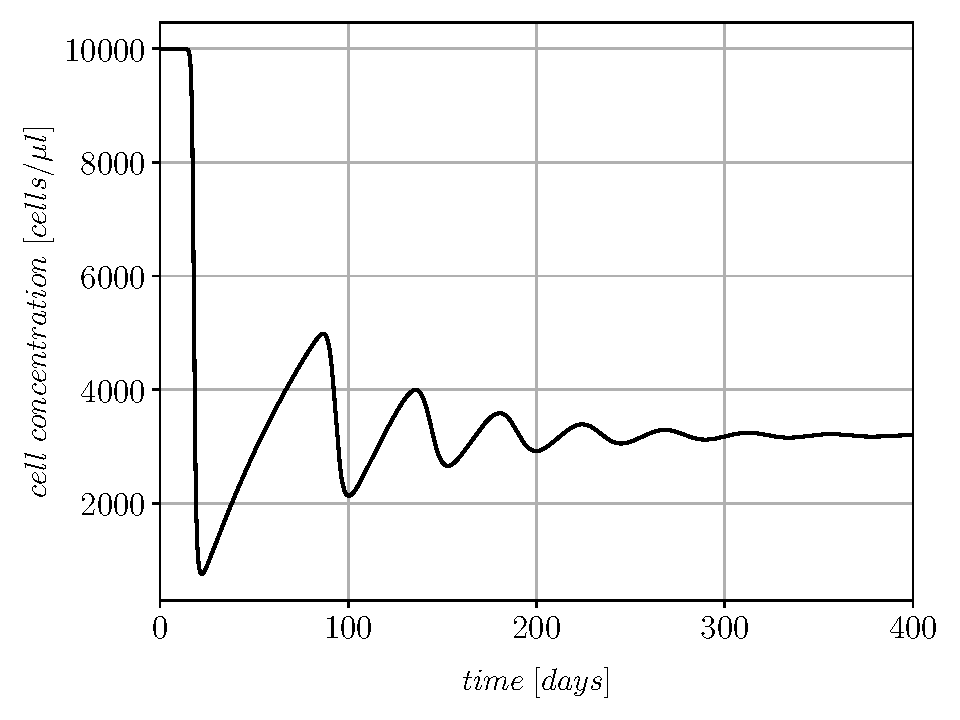
\includegraphics[width=\textwidth]{images/eRT_0_alpha_0/untreated_T.pdf}
        \caption[]%
        {{\small Uninfected CD4+ T cells}}    
        \label{fig1a:uninfected_T_cells}
    \end{subfigure}
    % \hfill
    % \begin{subfigure}[b]{0.3\textwidth}  
    %     \centering 
    %     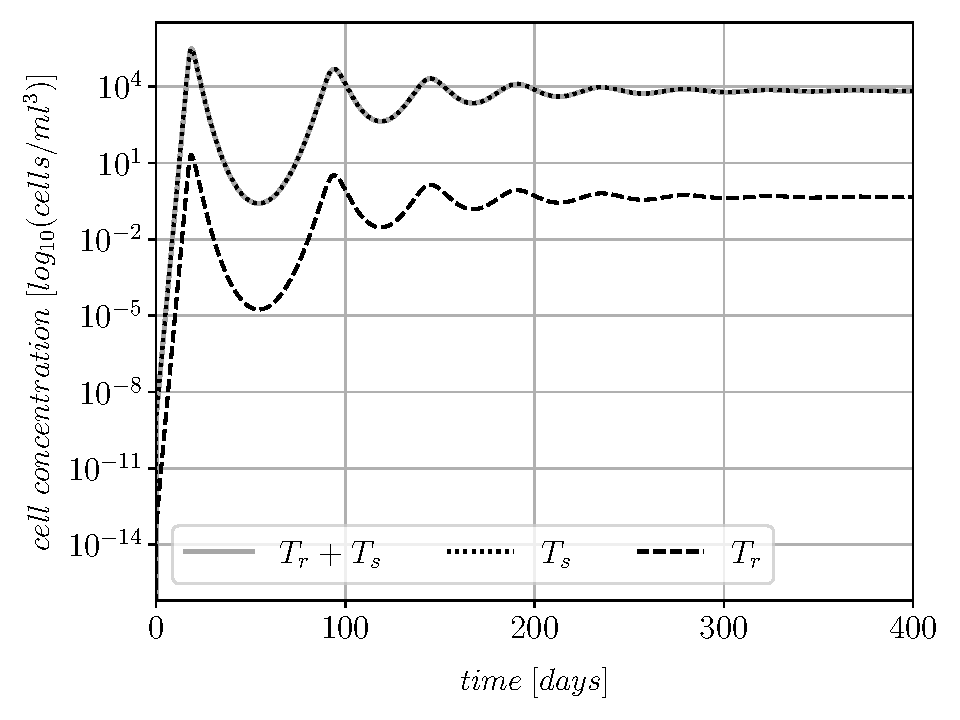
\includegraphics[width=\textwidth]{images/eRT_0_alpha_0/untreated_overview_infected_T.pdf}
    %     \caption[]%
    %     {{\small Infected CD4+ T cells}}    
    %     \label{fig1b:infected_T_cells}
    % \end{subfigure}
    % \vskip\baselineskip
    \begin{subfigure}[b]{0.475\textwidth}   
        \centering 
        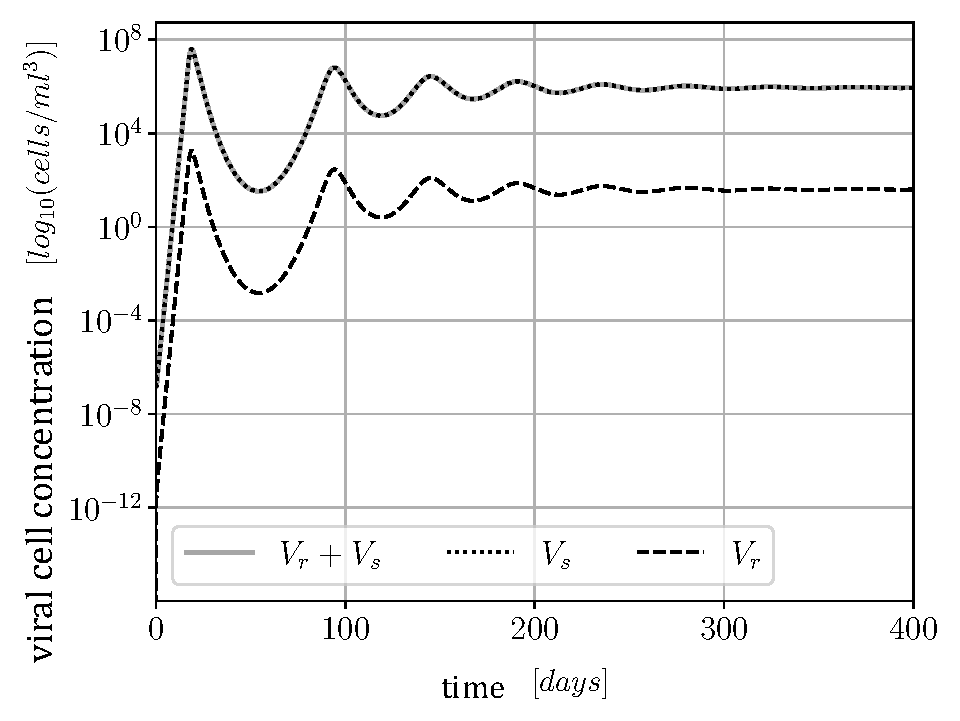
\includegraphics[width=\textwidth]{images/eRT_0_alpha_0/untreated_overview_V.pdf}
        \caption[]%
        {{\small Viral load}}    
        \label{fig1c:viral_load}
    \end{subfigure}
    \caption[]{Simulation of the pretreatment evolution of an initial HIV infection.
    For the inital state, the following values are assumed: $T(0) = 10^{6} \, \text{ml}^{-1}$, $T_s(0) = 0 \, \text{ml}^{-1}$, 
    $T_r(0) = 0 \, \text{ml}^{-1}$, $V_s(0) = 10^{-6} \, \text{ml}^{-1}$ and $V_r(0) = 0 \, \text{ml}^{-1}$ \cite{perelson1993dynamics}.}
    \label{fig:untreated}
\end{figure}

We assume that at this point of the disease, the infection is recognized and HAART is prescribed.
With a presumed low resistance level of $\alpha = 0.2$, the therapy is quantified by $\varepsilon_{RT}^{s} = 0.4$ and $\varepsilon_{PI}^{s} = \varepsilon_{PI}^{r} = 0$.
As initial values, the steady states of the pretreatment simualtion are chosen.\newline
The numerical results, given in figure \ref{fig2:treated_eRT_04_alpha_02}, show that indeed the therapy lowers the viral load and allows the 
number of uninfected immune cells to rise again.

\begin{figure}
    \centering
    \begin{subfigure}[b]{0.475\textwidth}
        \centering
        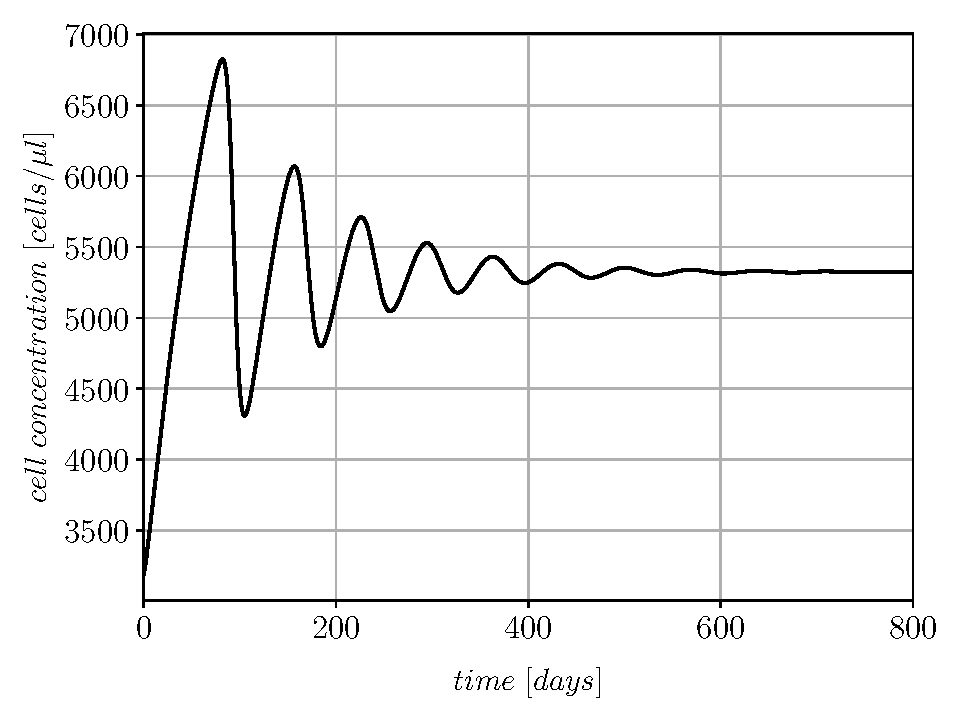
\includegraphics[width=\textwidth]{images/eRT_04_alpha_02/treated_T.pdf}
        \caption[]%
        {{\small Uninfected CD4+ T cells}}    
        \label{fig2a:uninfected_T_cells}
    \end{subfigure}
    % \hfill
    % \begin{subfigure}[b]{0.3\textwidth}  
    %     \centering 
    %     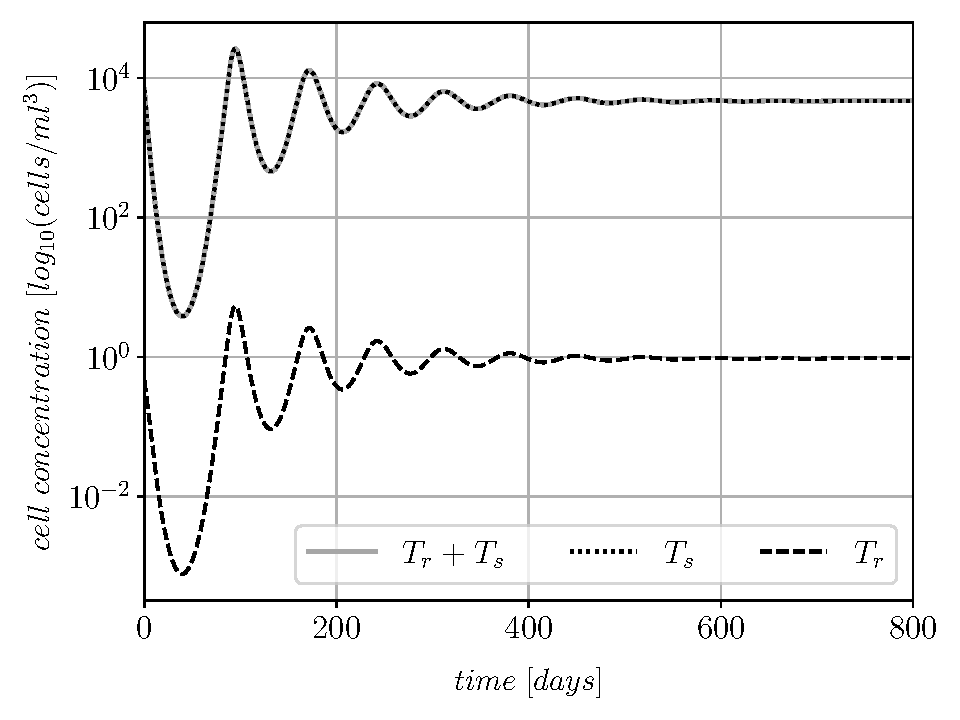
\includegraphics[width=\textwidth]{images/eRT_04_alpha_02/treated_overview_infected_T.pdf}
    %     \caption[]%
    %     {{\small Infected CD4+ T cells}}    
    %     \label{fig2b:infected_T_cells}
    % \end{subfigure}
    % \vskip\baselineskip
    \begin{subfigure}[b]{0.475\textwidth}   
        \centering 
        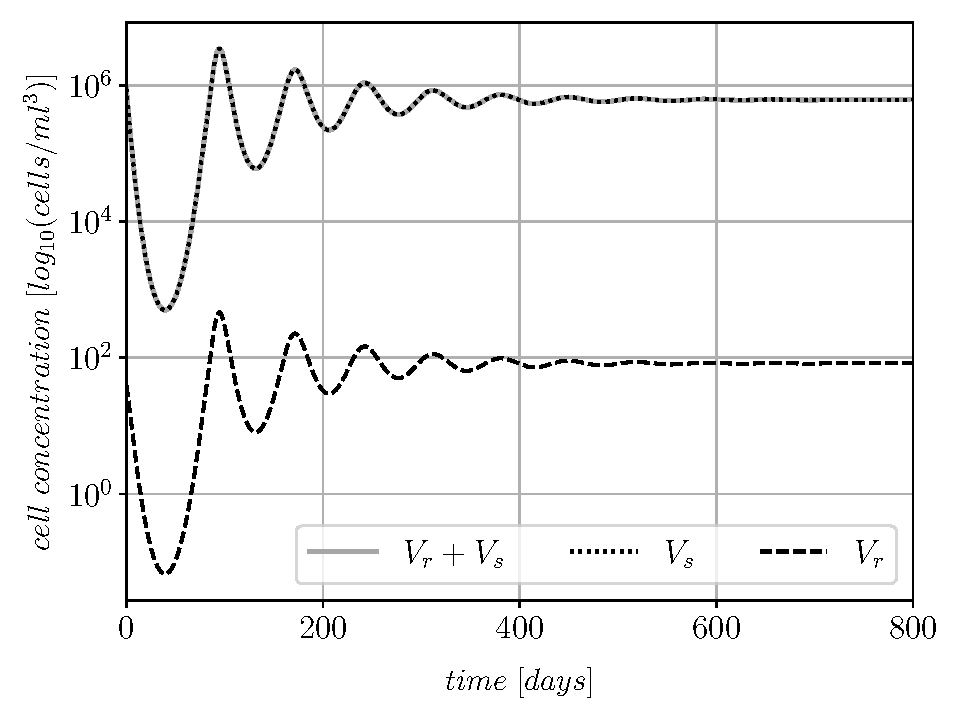
\includegraphics[width=\textwidth]{images/eRT_04_alpha_02/treated_overview_V.pdf}
        \caption[]%
        {{\small Viral load}}    
        \label{fig2c:viral_load}
    \end{subfigure}
    \caption[]{Simulation of the evolution of an HIV infection under HAART.
    It is $\varepsilon_{RT}^s = 0.4$, $\varepsilon_{RT}^r = \alpha \varepsilon_{RT}^s$ with $\alpha = 0.2$ and 
    $\varepsilon_{PI}^s = \varepsilon_{PI}^r = 0$.
    The steady states of the preceding pretreatment simulation are used as initial values, i.e. $T(0) = 3.19 \times 10^{5} \, \text{ml}^{-1}$, 
    $T_s(0) = 6.81 \times 10^{3} \, \text{ml}^{-1}$, $T_r(0) = 0.46 \, \text{ml}^{-1}$, $V_s(0) = 8.88 \times 10^{5} \, \text{ml}^{-1}$ 
    and $V_r(0) = 39.95 \, \text{ml}^{-1}$ \cite{perelson1993dynamics}.}
    \label{fig2:treated_eRT_04_alpha_02}
\end{figure}

An essential feature of the model is the development of the steady states as a function of medication efficacy of the drug-sensitive strain.
This is demonstrated in figure \ref{fig3:evolution_over_epsilon}, where the CD4+ T cell and viral count are plotted over $\varepsilon_s$.
From diagram \ref{fig3a:uninfected_T_cells}, it can be seen that for low values of $\varepsilon_s$, HAART achieve an increase in the 
number of uninfected target cells.
However, above a certain point, this growth saturates and the concentration remains on a constantly high level.
We denote this point of maximal efficacy by $\varepsilon_{s,max}$. 
For the given set of model parameters, its value is $\varepsilon_{s,max} \approx 0.5$.
A similar behaviour can be observed on the virus side, shown in figure \ref{fig3c:viral_load}.
In the lower $\varepsilon_s$ regime, the total virus count behaves reciprocally proportional to drug efficacy.
For $\varepsilon_{s,max} \leq \varepsilon_{s}$ this reduction halts after a large drop and the number of free virus settles in a steady state.\newline
% Obviously, further increasing the dose or potency of the drug does not lead to an improvement.\newline
An explanation for this behaviour can be found by investigating the evolution of the viral load more closely.
While the inital success of the therapy is based on pushing the number of $V_s$ beneath the threshold of detectability, 
the point of saturation sets in when the concentration of the drug-resistant strain erraticly increases.
The following consistency of the infection arises from two factors.
Firstly, due to the low level of $V_s$ no new mutations emerge.
Secondly, RTIs inhibit novel infections of the target cells and hence, the number of drug-resistant virus remains on a stable level.
Note, that due to the definition $\varepsilon_{RT}^r = \alpha \varepsilon_{RT}^s$, antiretroviral medications are not in- but only less 
efficient in attacking drug-resistant viruses (as long as $\alpha > 0$).\newline
The quintessence hereof is, that above a certain value $\varepsilon_{s,max}$, simply increasing dose or potency of antiretroviral drugs does not automatically 
result in an improvement of the therapy but only in an enhancement of their side effects.
At the same time, this turning point depends on the model parameters, i.e. on each patient individually.
This finding emphasises the necessity to personalize the model.

\begin{figure}
    \centering
    \begin{subfigure}[b]{0.475\textwidth}
        \centering
        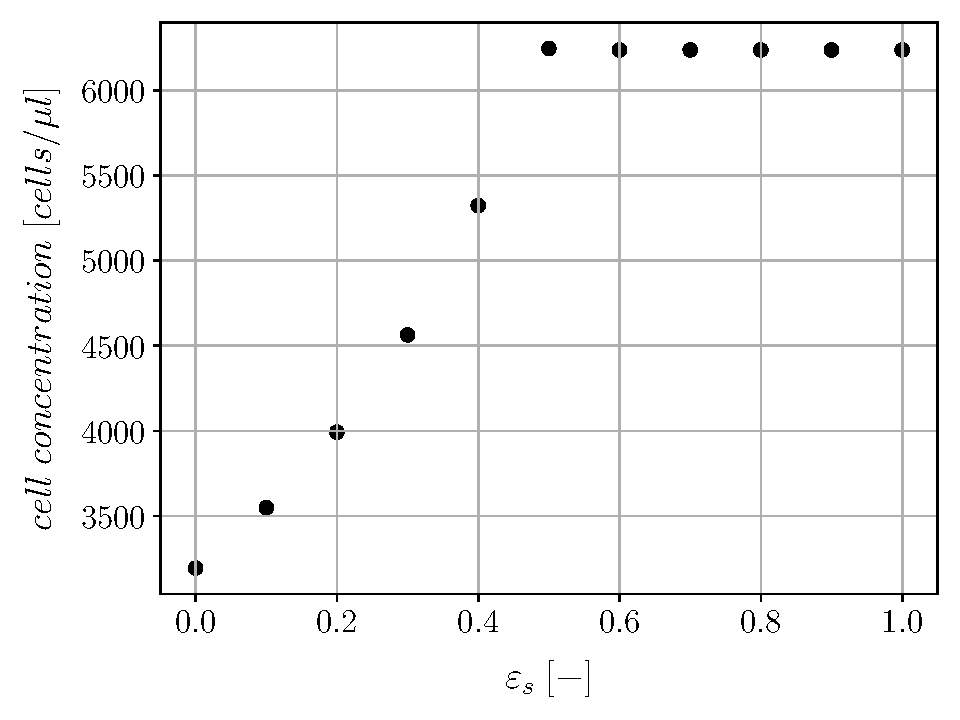
\includegraphics[width=\textwidth]{images/evolution_over_epsilon/treated_T.pdf}
        \caption[]%
        {{\small Uninfected CD4+ T cells}}    
        \label{fig3a:uninfected_T_cells}
    \end{subfigure}
    % \hfill
    % \begin{subfigure}[b]{0.3\textwidth}  
    %     \centering 
    %     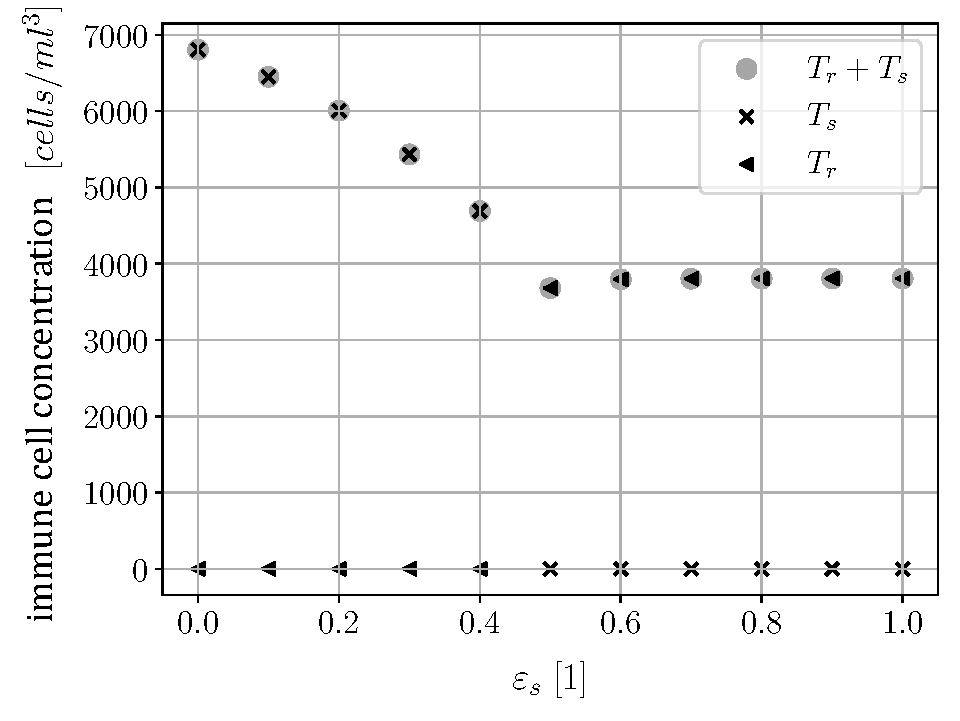
\includegraphics[width=\textwidth]{images/evolution_over_epsilon/treated_overview_infected_T.pdf}
    %     \caption[]%
    %     {{\small Infected CD4+ T cells}}    
    %     \label{fig3b:infected_T_cells}
    % \end{subfigure}
    % \vskip\baselineskip
    \begin{subfigure}[b]{0.475\textwidth}   
        \centering 
        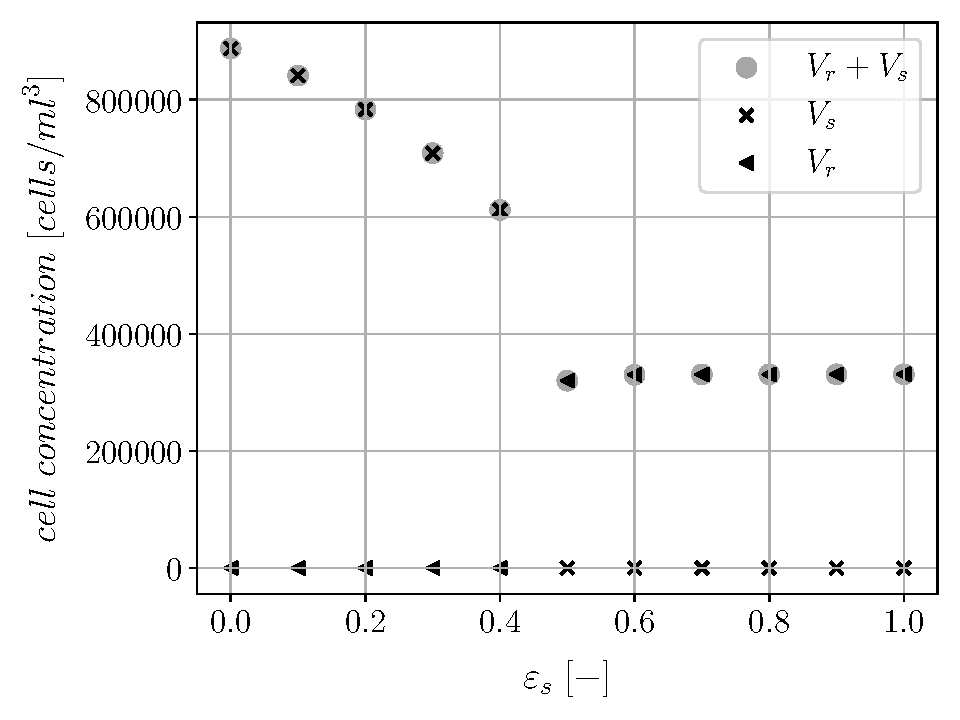
\includegraphics[width=\textwidth]{images/evolution_over_epsilon/treated_overview_V.pdf}
        \caption[]%
        {{\small Viral load}}    
        \label{fig3c:viral_load}
    \end{subfigure}
    \caption[]{The above diagrams show the evolutoin of the HIV infection in dependency of the drug efficacy parameter $\varepsilon_s$.
    In the considered case, it is $\varepsilon_{PI}^s =0$, $\varepsilon_{RT}^s = 0.4$ and $\alpha = 0.2$.
    Hence, the simulations basically demonstrate the impact of RTIs.}
    \label{fig3:evolution_over_epsilon}
\end{figure}

\subsection{The Optimal Control Problem}
\label{subsec:Model_OptControl}

An optimal therapy is one, that maximizes the level of CD4+ T cells while deploying as little drugs as possible.
Here, we assume that more and stronger drugs, i.e. higher $\varepsilon_s$ and $\varepsilon_r$, are associated with heavier 
side effects. 
Further, as shown in the preceding subsection \ref{subsec:Model_DynModel}, above a certain threshold efficacy $\varepsilon_{s,max}$, the effects of 
HAART saturate.\newline
From mathematical point of view, finding an ideal therapy can be formulated as an optimal control problem.
For this, we quantifiy the cost of HAART in the time interval $[t_0,t_1]$, by the functional

\begin{align}
    J(\mathbf{\varepsilon}) = \int_{t_0}^{t_1} \left(T^2(t) - A_1 \varepsilon_{s}^2 - A_2 \varepsilon_{r}^2\right) dt
    \label{equ:cost_function}
\end{align}

where $\mathbf{\varepsilon} = (\varepsilon_s, \varepsilon_r)^T \in [0,1]^2$ are the control parameters and $A_1$ and $A_2$ their 
weight constants \cite{adams2005hiv,wu2010game}.
The second term represents the cost of the drug treatment, which is to be minimized.
Hence, we seek an optimal control $\mathbf{\varepsilon}_{opt}$, such that

\begin{align}
    \mathbf{\varepsilon}_{opt} = \underset{\mathbf{\varepsilon} \in [0,1]^2}{\arg\max}\, (J(\mathbf{\varepsilon}_{opt})) \text{.}
    \label{equ:opti_control}
\end{align}

\section{The Data}
\label{sec:data}

Previously, we have seen that the dynamics of a treated HIV infection is described by a set of nonlinear differential equations.
Finding the most efficient HAART while minimizing its side-effects, requires a personalization of the model.
This is achieved by estimating the parameters $\mathbf{m}$ from blood measurements.
Their acquisition and expected inaccuracies is discussed in this section.\par
Each new drug therapy is preceded by a preparatory phase during which the total viral cell concentration $V_{tot}(t) = V_r(t) + V_s(t)$ and the CD4+ T cell count $T_{tot}(t) = T(t) + T_r(t) + T_s(t)$ are recorded.
In this 8 weeks lasting period, the patient can, obviously, not be left untreated. 
She or he receives suboptimal therapy, reusing $\varepsilon_{RT}^s = 0.4$ and $\varepsilon_{PI}^s = 0.0$ from above.
With $\alpha = 0.2$, it is $\varepsilon_{RT}^r = 0.08$ and $\varepsilon_{PI}^r = 0.0$.\\
In the previous discussion, we have learned that the initial treatment phase is highly dynamic.
Hence, the measurement schedule has to be designed such that the examinitions are carried out at intervalls, close enough to track these oscillations.
At the same time, one wants to make as few blood plasma tests as possible since they are not only time consuming and expensive but also an additional physical and psychological burden for the patient.
A good balance is, a one-week interval where once a week, two blood plasma samples are taken.
One is used to determine $T_{tot}(t)$, the other for $V_{tot}(t)$.\newline
However, determining the exact amount of virus and immune cells from blood plasma is not trivial.
The smallest variations in the sampled plasma volume or too long periods between plasma sampling and final analysis during which viruses can inhibit, are only two factors that potentially contaminate the data with errors.
In addition hereto, other aspects such as errors introduced by the laboratory tools, further reduce the reliability of the measurements.
Having this in mind, we can interpret the final $8$-dimensional observation vectors $\mathbf{T}_{obs} \in \mathbb{R}^8$ and $\mathbf{V}_{obs} \in \mathbb{R}^8$ with $\mathbf{T}_{obs,i} = T_{obs}(t_i)$ and $\mathbf{V}_{obs,i} = V_{obs}(t_i)$, respectively, and for $i \in [0,7]$, as realizations of random variables.
Their statistics are described in terms of the following conditional distributions
\begin{align}
    p(\mathbf{T}_{obs}|\mathbf{m}) = 
    \begin{cases}
        0 \quad & T_{obs}(t_i) < 0\\
        \mathcal{N}(\mathbf{T}_{tot}, C_{D_T}) \; & \text{else}
    \end{cases} \quad\quad ,i \in [0,7]
    \label{equ:prior_D_T}
\end{align}
\begin{align}
    p(\mathbf{V}_{obs}|\mathbf{m}) = 
    \begin{cases}
        0 \quad & V_{obs}(t_i) < 0\\
        \mathcal{N}(\mathbf{V}_{tot}, C_{D_V}) \; & \text{else}
    \end{cases} \quad\quad ,i \in [0,7]
    \label{equ:prior_D_V}
\end{align}
which encode the prior knowledge that we have about the measurements.
Firstly, negative cell concentrations are unrealistic and hence, their probability is set to 0.
For positive values, we assume that the measurement errors are distributed normally with mean $\mathbf{T}_{tot}(\mathbf{m}) = [T_{tot}(t_0,\mathbf{m}),\dots,T_{tot}(t_7,\mathbf{m})]^T$ and $\mathbf{V}_{tot}(\mathbf{m}) = [V_{tot}(t_0,\mathbf{m}),\dots,V_{tot}(t_7,\mathbf{m})]^T$, respectively.
Since single samples are independent of each other, the covariance matrices $C_{D_T}$ and $C_{D_V}$, have only non-zero diagonal entries.
These are the variances in each measurement and describe the observational uncertainty that we have about the value.
Determining viral cells in blood plasma is significantly more challenging that tracking the body's own immune cells.
This difference is included in the probability distributions by setting $C_{{D_V},jj} > C_{{D_T},jj}$, $j \in [0,7]$. 
We choose $C_{{D_T},jj} = 200$ and $C_{{D_V},jj} = 250$.\\
Statistics \ref{equ:prior_D_T} and \ref{equ:prior_D_V} can further be summarized to describe the joint distribution over all observations, i.e. $p(\mathbf{d}_{obs}|\mathbf{m})$ with $\mathbf{d}_{obs} = \{\mathbf{T}_{obs},\mathbf{V}_{obs}\}$.
Since $\mathbf{T}_{obs}$ and $\mathbf{V}_{obs}$ are derived from independent samples, their joint distribution simplifies to
\begin{align}
        p(\mathbf{d}_{obs}|\mathbf{m})
        = p(\mathbf{T}_{obs},\mathbf{V}_{obs}|\mathbf{m}) 
        = p(\mathbf{T}_{obs}|\mathbf{m})p(\mathbf{V}_{obs}|\mathbf{m}) 
        = \frac{1}{4\pi^2 \sqrt{|C_{D_T}||C_{D_V}|}}e^{\mathbf{\chi}(\mathbf{m})}
    \label{equ:prior_D}
\end{align}
where $|\cdot|$ is the determinat of a matrix and
\begin{align}
    \begin{split}
        \mathbf{\chi}(\mathbf{m}) = -\frac{1}{2}&\bigr((\mathbf{T}_{obs} - \mathbf{T}_{tot}(\mathbf{m}))^T C_{D_T}^{-1}(\mathbf{T}_{obs} - \mathbf{T}_{tot}(\mathbf{m})) 
        \\&+ (\mathbf{V}_{obs} - \mathbf{V}_{tot}(\mathbf{m}))^T C_{D_V}^{-1}(\mathbf{V}_{obs} - \mathbf{V}_{tot}(\mathbf{m}))\bigl).
    \end{split}
    \label{equ:prior_D_exp}
\end{align}
Since we do not have access to real data, we work with artifical data instead.
For this, we simulate the means $T_{tot}(t_i)$ and $V_{tot}(t_i)$ by solving the forward model \ref{equ:HIVmodel} at times $t_i \in \{7i|i \in [0,7]\}$.
Note, that to synthesize the data, we have to predefine the set of true parameters $\mathbf{m}_{true}$.
In the following, we assume that the earlier used values, listed in table \ref{tab:init_parameters}, are the true parameters which we want to recover from blood measurements.
\section{The Methods}
\label{sec:methods}

After discussing the acquistion of blood measurement data, this section is devoted to consider the model parameters, the inverse problem itself and finally appropriate solution methods in more detail.

\subsection{Probabilistic Formulation of Prior Knowledge and Bayes' Theorem}

First of all, the aim is to find the model parameters $\mathbf{m} = \{\lambda, \gamma, k_s, k_r, N_s, N_r, \delta, c\} \in \mathbb{R}^8$ which best explain the measured cell loads $\mathbf{d}_{obs} = \{\mathbf{T}_{obs},\mathbf{V}_{obs}\}$.
Generally, the exact values of the parameters are unknown and therefore, are modelled by probability distributions.
In doing so, the following prior knowledge can be incorporated.
Firstly, from basic physics and biology it can be inferred that the model parameters are always non-negative.
Secondly, due to extensive, preceding clinical tests on other HIV patients as well as on animals, the rough order of magnitude of the parameters is known.
These prior values are assumed to be the means around which the parameters deviate with a certain variance.
Perelson et al. \cite{perelson1993}, for instance, derive from the infection dynamics that it is reasonable to assume that $k_s$ is uniformly distributed over the interval $(1.2\times 10^{-8}, 3.6\times 10^{-8})\;\text{ml day}^{-1}$.
Similar behaviour can be suggested for the drug-resistant population and $k_r \sim \mathcal{U}(1.0\times 10^{-8}, 3.0\times 10^{-8})\;\text{ml day}^{-1}$. 
Further, the numbers $N_s$ and $N_r$ of viruses that infected CD4+ T cells release after bursting, are again distributed uniformly over $(2000,4000)$ and $(1000,3000)$, respectively.\newline
As Rong et al. \cite{rong2007emergence} before, we model the remaining $4$ parameters as random variables with an asymmetric triangular distribution.
The latter is defined by three values $(lb,p,ub)$ where $lb$ and $ub$ are lower and upper bound, respectively, and $p$ is the peak value.
For a random variable $x$, this statistic is defined as
\begin{align}
    x \sim \mathcal{T}(lb,p,ub) = 
    \begin{cases}
        \frac{2(x-lb)}{(ub-lb)(p-lb)}&,\; lb \leq x \leq p\\ 
        \frac{2(ub-x)}{(ub-lb)(ub-p)}&,\; p < x \leq ub\\
        0 \;&, x < lb \text{ and } ub < x\\
    \end{cases}
    \label{equ:asy_tri_distribution}
\end{align}
With that, the death rate $\gamma$ of uninfected immune cells is drawn from $\mathcal{T}(0.005, 0.01, 0.016)\;\text{day}^{-1}$.
% The first value describes the lower value, $0.01\text{ day}^{-1}$ is the peak value and the last one sets an upper bound.
In \cite{rong2007emergence} it is further stated, that the immune cell birth rate $\lambda$ is a $T(0)$ multiple of $\gamma$.
Hence, following the discussion from the previous section and using $T(0) = 3.19\times 10^5 \text{ ml}^{-1}$, it is $\lambda \sim \mathcal{T}(1.595, 3.19, 5.104)\times 10^4\;\text{ml}^{-1}\;\text{day}^{-1}$.
The viral clearnace rate $c$ is sampled from another asymmetric traingular distribution with lower and upper bounds $9.1 \text{ day}^{-1}$ and $36 \text{ day}^{-1}$, respectively, and peak $23 \text{ day}^{-1}$.
Finally, the death rate $\delta$ of infected cells is drawn from $\mathcal{T}(0.25,1,1.5)\;\text{day}^{-1}$.\newline
Summarizing the information about the single and mutually independent model parameters, their joint probability distribution takes the form
\begin{align}
    p(\mathbf{m}) = p(\lambda)p(\gamma)p(k_s)p(k_r)p(N_s)p(N_r)p(\delta)p(c).
    \label{equ:prior_M}
\end{align}
After representing the prior knowledge in data and model space in form of probability distributions, the next step can be taken and the inverse problem itself is considered.
First of all, the problem, with its eight unknown model parameters $\mathbf{m} \in \mathbb{R}^8$, and the eight observations $\mathbf{d}_{obs} \in \mathbb{R}^8$ is even-determined.
In section \ref{sec:data}, it has been mentioned that \textit{as few as possible} blood plasma test should be conducted.
Here, the minimal number is set by the necessity to generate at least as many observations as unknown parameters in order to avoid an over- or under-determined problem.\\
Following this, the inverse problem has to be formulated.
Generally, there are three possibilities namely defining the inversion as an optimization problem, a deterministic least-squares problem or a Bayesian inverse problem.
The first option is based on approximating a problem-dependent misfit function. This approach is appropriate for a weakly non-linear forward problem.
Opposed to that, a deterministic least-square problem solves the root-mean square misfit function for a linear forward model.
Since this includes the inversion of possibly singular matrices, one has to incorporate prior knowledge as well as regularization techniques (equivalent to include artificial prior knowledge). 
Last but not least, a Bayesian inverse problem derives the a posterior model distribution $p(\mathbf{m}|\mathbf{d}_{obs})$ from the prior distributions in model and data space with Bayes theorem.
Following this, computationally expensive Monte Carlos Methods are used to sample from the posterior distribution since the latter is generally not given explicitly.
The finally selected model is then for instance the \textit{maximum a posterior model} $\mathbf{m}_{MAP}$.
In a special case, where the forward model is linear and both prior distributions are Gaussian, the probabilistic approach of Bayes can be formulated as a least-squares problem and the posterior distribution can be defined explicitly.\\
However, the fact that the forward model for the HIV dynamics is non-linear and none of the prior distributions is purely Gaussian, directly excludes the least-square approach.
Further, one could either choose to linearize the forward model and define the problem as an optimization or to formulate it as a Bayes inverse problem.
An often mentioned disadvantages of the latter is, that sampling from a distribution with Monte Carlo Methods is computationally expensive.
Apart from that, Bayes approach has no inherent limitation and even has the strong advantage to directly include an uncertainty quantification since the likelihood is directly attached to each model as a measure of plausibility.\\
Hence, despite the high computational cost, it is reasonable to formulate the problem as a Bayes inversion.
It is 

\begin{align}
    p(\mathbf{m}|\mathbf{d}_{obs}) = \frac{p(\mathbf{d}_{obs}|\mathbf{m})p(\mathbf{m})}{p(\mathbf{d}_{obs})} \quad .
\end{align}

where we aim on copmuting the maximum likelihood estimation of $p(\mathbf{m}|\mathbf{d}_{obs})$.

\subsection{Sampling with Markov Chain Monte Carlo Method}

As mentioned above, in most cases the posterior model distribution $p(\mathbf{m}|\mathbf{d}_{obs})$ can not be computed analytically and hence, Bayes approach has to be equipped with an algorithm to sample from it.
A very simple choice would be a systematic grid search in the model space.
However, since it heavily suffers from the curse of dimensionality, Monte Carlo Methods (MCM) are more appropriate.
Generally speaking, these methods are capable of numerically solving a broad class of computational problems by repeated random sampling.
Here, we use MCM to compute samples of the model posterior distribution.
For this, a Markov Chain is constructed whose equilibrium distribution equals $p(\mathbf{m}|\mathbf{d}_{obs})$.
The arising class of algorithms are called Markov Chain Monte Carlo (MCMC) methods.
While simple grid searches deterministically scan through the complete model space, MCMC perform random searches.
They try to avoid regions in the search space that are less relevant than other.
Meaningful models are identified by taking the prior knowledge into account.\newline
A special MCMC algorithm is the so-called Simulated Annealing (SA).
Based on the Metropolis-Hasting acceptance rule, it samples from a modified posterior probability distribution $p_T(\mathbf{m}|\mathbf{d}_{obs})$.
Due to this modification of the distribution, the algorithm starts sampling from a very broad $p_T(\mathbf{m}|\mathbf{d}_{obs})$.
In the course of the SA sampling, the peaks of the modified distribution become more and more distinct.
For a sufficiently slow transition from the broad $p_T(\mathbf{m}|\mathbf{d}_{obs})$ to the distinct one, convergence towards the global maximum-likelihood model is guaranteed.\\
Hence, the solution of the inverse problem is automatically the maximum likelihood model $\mathbf{m}_{MAP}$.
As mentioned earlier, Bayes approach does not require any additional uncertainty assessment.
\section{Discussion and Conclusion}
\label{sec:Dis}

A crucial aspect of the success of the introduced approach is the reliability of the observations $V_{obs}$.
To diminish measurement errors and reduce the effect of outliers one could extract multiple samples of plasma every other week and average the viral loads.\\
In addition hereto, the prior distribution in model space $p(\mathbf{d}_{obs}|\mathbf{m})$ has inconsistencies relating to the independence of the observations.
As already discussed in chapter \ref{sec:Data}, dependent on the value of each $V_{obs}(t_i)$, the joint probability distribution might be set to 0.
At the same time, if each $V_{obs}(t_i) > 0$, the measurements are assumed to be independent.
Hence, different prior probability distributions should be investigated.\\
Generally, the prior distributions in model and data space are heavily subjective.
In order to perfectly model the prior knowledge it would be reasonable to analyse the choices of the variance $\sigma_D^2$ and $Var[\mathbf{m}]$ as well as the distributions themselves.\\ \\
Although, some aspects of the introduced methodology still leave freedom for improvement, the presented work lays the foundation for an individually tailored drug treatment and to find the optimal drug adjustment for each patient.
\section{Discussion}
\label{sec:dis}


% A crucial aspect of the success of the introduced approach is the reliability of the observations $V_{obs}$.
% To diminish measurement errors and reduce the effect of outliers one could extract multiple samples of plasma every other week and average the viral loads.\\
% In addition hereto, the prior distribution in model space $p(\mathbf{d}_{obs}|\mathbf{m})$ has inconsistencies relating to the independence of the observations.
% As already discussed in chapter \ref{sec:Data}, dependent on the value of each $V_{obs}(t_i)$, the joint probability distribution might be set to 0.
% At the same time, if each $V_{obs}(t_i) > 0$, the measurements are assumed to be independent.
% Hence, different prior probability distributions should be investigated.\\
% Generally, the prior distributions in model and data space are heavily subjective.
% In order to perfectly model the prior knowledge it would be reasonable to analyse the choices of the variance $\sigma_D^2$ and $Var[\mathbf{m}]$ as well as the distributions themselves.\\ \\
% Although, some aspects of the introduced methodology still leave freedom for improvement, the presented work lays the foundation for an individually tailored drug treatment and to find the optimal drug adjustment for each patient.
\section{Conclusion and Outlook}
\label{sec:con}
\newpage
\bibliographystyle{abbrv} 
\bibliography{chapter/References.bib}
\newpage


\end{document}